\documentclass[full.tex]{subfiles}

\graphicspath{ {assets/note0/} }
\newcommand{\notenum}{0}


\begin{document}
    \thispagestyle{firstpage}
    \vspace*{2\baselineskip}
    \section*{Introduction}
    
    \begin{center}
         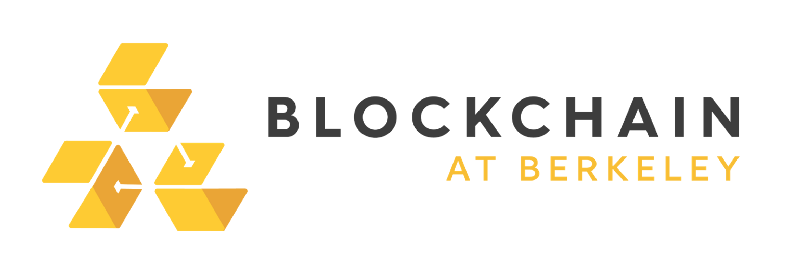
\includegraphics[scale=0.5]{bab}
    \end{center}
     
     
    After taking Blockchain at Berkeley's Spring 2017 Introduction to Cryptocurrencies DeCal, I decided to make a set of notes to reinforce my learning and also to compile the core ideas of blockchain onto an easily readable format. Big thanks to the wonderful lecturers, officers, and other folks at Blockchain at Berkeley for getting me hyped. I have structured this set of notes after their lecture slides. This set of notes started off as a personal passion project of mine but has since garnered the interest of Blockchain at Berkeley executive staff, namely DeCal lecturer Nadir Akhtar. This project has been a collaborative effort ever since, and will be provided as complementary material to future DeCal offerings.
    
    There will be bugs, shaky facts, and some hand-wavy stuff. Be warned! In any case, if you do find yourself reading this, I hope you enjoy! -- \textit{Rustie Lin} 
    
    \medskip
    
    ``how do i get bigger than Bigg but not as big as huge" -- \textit{Nadir Akhtar}
    
    \bigskip
    
    \noindent \textbf{\textit{Guidelines for use:}}
    
    These notes are based on the Spring 2017 edition of Blockchain at Berkeley's ``Introduction to Cryptocurrencies and Blockchain" student-run class. (For any non-Berkeley students: these courses are referred to as DeCals, short for ``Democracy at Cal," exclusively student-run courses.) Any updates to the course, including but not limited to material or structure, are not necessarily be reflected within these notes.
    \begin{itemize}
        \item Each of these notes corresponds to a specific lecture. It may help to read the note before going through the lecture, or go through the lecture before going through the notes, or use one of the two exclusively. We have no clue! You let us know what works best for you, we're curious ourselves!
        \item All of the crypto/blockchain material comes from Blockchain at Berkeley. Notes will contain about just as much information as lectures, profoundly overlapping in information. Again, these notes are merely a different way to present the information generated by Blockchain at Berkeley. A few tweaks in wording may have been made based on our judgment, details may have been added or omitted, but all main ideas remain.
        \item Every note will end with a page on ``Key Terms," composed of any bolded terms within the given note. These Key Terms will either be important crypto/blockchain terms or terms perhaps unfamiliar to the average reader. Terms will be organized alphabetically. While reading the Key Terms alone may give you a quick \textit{sense} of the content, they will hardly give you an understanding.
        \item References to various outside sources are included in a separate file from all notes. Any uncited information (almost everything in these notes) can be assumed to come from Blockchain at Berkeley. We are not validating all information in these notes; responsibility for any improper or false information belongs to the source of info. Don't shoot the messenger. One note, definitions for Key Terms are rarely word-for-word from Blockchain at Berkeley. (In other words, they're mostly paraphrased or even made from scratch based on personal knowledge.)
    \end{itemize}
    
    \newpage
    \thispagestyle{firstpage}
    \vspace*{2\baselineskip}
    \section*{Key Terms}
    \noindent Below is a working list of commonly used terms and their definitions in the Blockchain space.
    \begin{enumerate}
        \item \textbf{Bitcoin} --- A popular cryptocurrency existing purely as software. ``Bitcoin" (uppercase) refers to the protocol, software, and community; whereas, ``bitcoins" (lowercase) refers to the unit of currency. It is not backed by any asset or regulated by any central entity. (See: \textit{Decentralized, Distributed})
        \item \textbf{Blockchain} --- An immutable and distributed database that maintains a growing list of records. Blockchains are used to safely and securely record transactions between parties. Originally designed to make Bitcoin possible.
        \item \textbf{Cryptocurrency} --- A digital currency in which encryption techniques are used to regulate the generation of units and currency and verify the transfer of funds, operating independently of a central bank.
        \item \textbf{Decentralized} --- A characteristic that ensures that no single entity has control over all the processing in a system.
        \item \textbf{Distributed} --- A characteristic that ensures that not all the processing in a system is done in the same location.
        \item \textbf{Trustless} --- A characteristic that ensures that a system or protocol can function without trusting a single entity. (e.g. Everyone has a copy of the Bitcoin ledger/blockchain, so users do not have to trust a single entity, organization, or third-party.)
        
        %%% QUESTION: Why did we include these specific terms and not transactions/blocks/miner/addresses? Just looking at the first lecture
    \end{enumerate}
\end{document}